\documentclass{Article}
\usepackage{graphicx}

\newtheorem{theorem}{Minimax}

\begin{document}

\title{Repeated Prisoner's Dilemma with Multi-Population Genetic Algorithms}
\author{John~Murrill}
\maketitle

\maketitle


\section{Introduction}
Below are multiple cases of the repeated game with varying payout structures. The standard format for all payout lists are CC, CD, DC, DD where C and D represent Cooperation or Defection. The first letter is the move of Player 1, the second letter is the move of Player 2. Payouts are listed according to each possible state the game can be in.

\subsection{Payout: \{1, 1\}, \{0, 10\}, \{10, 0\}, \{1, 1\}}
\begin{center}
Player 1 Strategy: 
  \begin{tabular}{c | c | c | c }
    0.173108 & 0.0307229 & 0.0385799 & 0.0215957 \\ \hline
    0.826892 & 0.969277 & 0.96142 & 0.978404 \\ \hline
  \end{tabular}
\end{center}
\begin{center}
Player 2 Strategy: 
  \begin{tabular}{c | c | c | c }
    0.394474 & 0.0428105 & 0.0560978 & 0.0299719 \\ \hline
    0.605526 & 0.95719 & 0.943902 & 0.970028 \\ \hline
  \end{tabular}
\end{center}
\begin{center}
These strategies lead to an eigenvector of:\\
\{0.00525789, 0.0577422, 0.0675418, 0.869458\}\\
\includegraphics[scale=0.5]{Oneone.png}
\end{center}
\newpage


\subsection{Payout: \{5, 5\}, \{0, 10\}, \{10, 0\}, \{1, 1\}}
\begin{center}
Player 1 Strategy: 
  \begin{tabular}{c | c | c | c }
    0.878337 & 0.153564 & 0.0402585 & 0.123226 \\ \hline
    0.121663 & 0.846436 & 0.959742 & 0.876774 \\ \hline
  \end{tabular}
\end{center}
\begin{center}
Player 2 Strategy: 
  \begin{tabular}{c | c | c | c }
    0.979694 & 0.24852 & 0.0782974 & 0.753991 \\ \hline
    0.0203062 & 0.75148 & 0.921703 & 0.246009 \\ \hline
  \end{tabular}
\end{center}
\begin{center}
These strategies lead to an eigenvector of:\\
\{0.270391, 0.155229, 0.129193, 0.445187\}\\
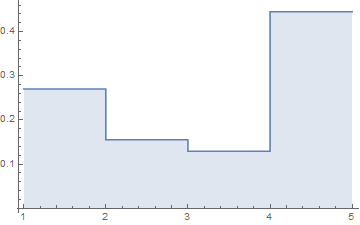
\includegraphics[scale=0.5]{fivefive.png}
\end{center}

\subsection{Payout: \{6, 6\}, \{0, 10\}, \{10, 0\}, \{1, 1\}}
\begin{center}
Player 1 Strategy: 
  \begin{tabular}{c | c | c | c }
    0.971696 & 0.0672063 & 0.0461624 & 0.936854 \\ \hline
    0.0283041 & 0.932794 & 0.953838 & 0.0631456 \\ \hline
  \end{tabular}
\end{center}
\begin{center}
Player 2 Strategy: 
  \begin{tabular}{c | c | c | c }
    0.975811 & 0.061588 & 0.0404697 & 0.93376 \\ \hline
    0.0241893 & 0.938412 & 0.95953 & 0.0662397 \\ \hline
  \end{tabular}
\end{center}
\begin{center}
These strategies lead to an eigenvector of:\\
\{0.844009, 0.0414005, 0.043781, 0.0708096\}\\
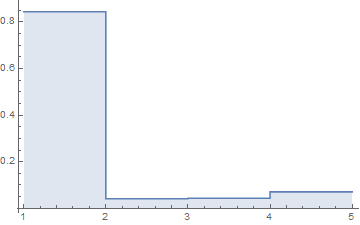
\includegraphics[scale=0.5]{sixsix.png}
\end{center}
\end{document}


